

\chapter{Basics of Private Key Encryption}
	
	\section{Limitations of Perfectly Secret Encryption}
		\begin{itemize}
			\item Thm of Shannon: In perfectly secret encryption key must be as long as the message and cannot be reused
			\item But: \textbf{Perfect Secrecy is an overkill!}
			\item Relaxation: Only consider adversaries with realistic computational power
			\item Also: \textbf{Is secrecy alone sufficient? What about other attacks?}
		\end{itemize}
		
	\section{Computational Security: Encryption}
		\begin{itemize}
			\item Back to the problem of secrecy with short keys
			\item \textbf{Idea:} Limit the runtime of adversaries
			\begin{itemize}
				\item We will relax the notion of perfect secrecy by considering only \textbf{computationally bounded} adversaries $\mathcal{A}$
				\item Assume that the runtime of adversaries is upper bounded by a realistic upper bound of $T$ operations, in practice often $T = 2^{80}$
			\end{itemize}
		\end{itemize}
	
	\section{Computationally Secure Encryption}
		Let's modify the definition of perfect secrecy to only account for $T$-bounded adversaries
		\begin{definition}[Computationally Secure Encryption: Attempt 1]
			An encryption scheme $(KeyGen,Enc,Dec)$ is $T-IND$ \textbf{secure}, if it holds for \textbf{every $T$-bounded adversary $\mathcal{A}$} that
			$$Pr[IND_{\mathcal{A}} = 1] = \frac{1}{2}$$
		\end{definition}
		
		Proper Definition: $T$-bounded adversaries with advantage $< \epsilon$
		\begin{definition}[Computationally Secure Encryption: Concrete Indistinguishability Security]
			An encryption scheme $(KeyGen,Enc,Dec)$ is $(T,\epsilon)-IND$ \textbf{secure}, if it holds for \textbf{every $T$-bounded adversary $\mathcal{A}$} that
			$$Pr[IND_{\mathcal{A}} = 1] < \frac{1}{2} + \epsilon$$
		\end{definition}
		\begin{center}
			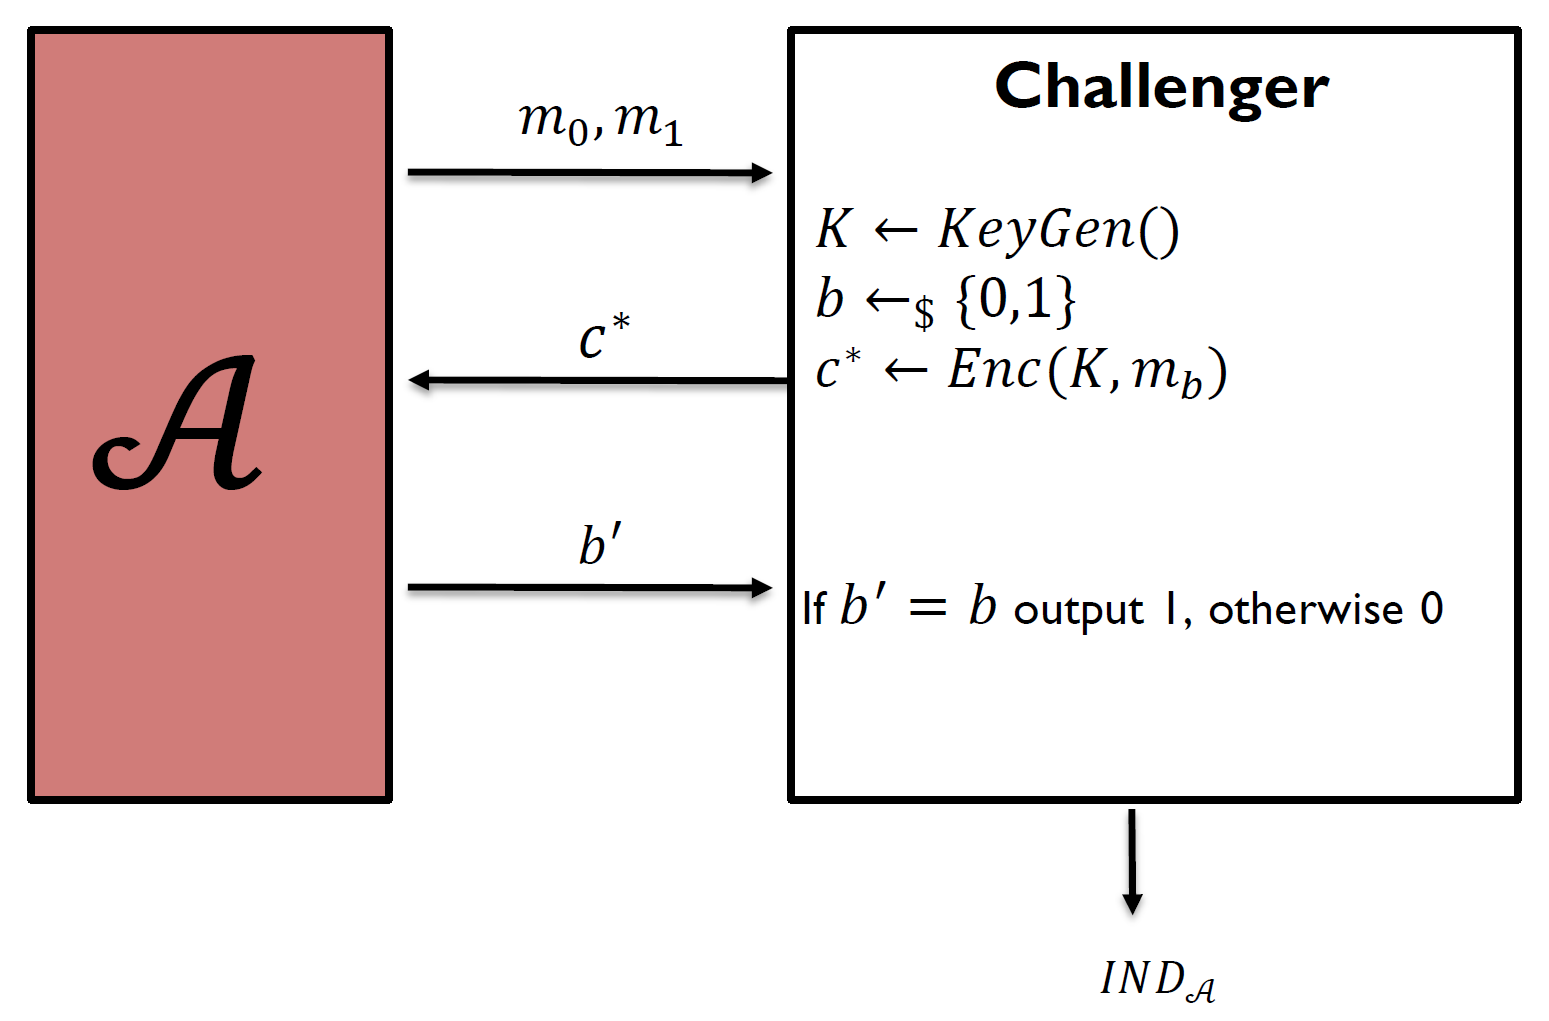
\includegraphics[width=120mm]{Graphics/Basics of Private Key Encryption/ComputationallySecureEncryption.png}\newline
		\end{center}
	
	\section{Concrete Security}
		\begin{itemize}
			\item How do we determine if a scheme is $(T,\epsilon)$-secure?
			\item In practice: Choose parameters of scheme such that \textbf{best known attack} with time complexity $T$ has advantage less than $\epsilon$
			\item In practice, often suggested parameters are $T = 2^{80}$ and $\epsilon = 2^{-60}$
			\item What is the unit of $T$?
			\begin{itemize}
				\item Milliseconds?
				\item Elementary CPU operations?
				\item CPU cycles?
			\end{itemize}
			\item What about other models of computation?
			\item Concrete security is inherently technology dependent!
			\item How can we argue about security in any \textit{reasonable} computational model?
		\end{itemize}
	
	\section{Asymptotic Complexity}
		\begin{itemize}
			\item Computational Complexity Theory!
			\item Recall: In complexity theory problems consist of an infinite number of instances
			\item The complexity of an algorithm solving a problem is measured as a function of the size of an instance, or more generally a \textit{size-parameter}
			\item E.g. sorting: Merge sort has complexity $\mathcal{O}(n \cdot log(n))$ to sort a list of $n$ elements
			\item Recall that we say that an algorithm is efficient, if it runs in time $poly(n)$
		\end{itemize}
		
	\section{Asymptotic Security}
		\begin{itemize}
			\item \textbf{Idea of asymptotic security:} Introduce a security parameter $\lambda$ which characterizes the hardness of breaking a scheme
			\item We only care about what happens when $\lambda \rightarrow \infty$
			\item $KeyGen$ now takes as explicit input security parameter $\lambda$, typically written in unary as $1^{\lambda}$
			\item Efficient computation: \textbf{probabilistic polynomial time (PPT) algorithms}, i.e. randomized algorithms running in time $poly(\lambda)$
			\item Thus efficient adversaries = PPT machines
			\item What about the advantage $\epsilon$?
			\item Exponentially small?
			\item Definitely smaller than $\frac{1}{poly(\lambda)}$ for every polynomial and sufficiently large $\lambda$!
		\end{itemize}

		\begin{definition}[Negligible Functions]
	    	A function $f: \mathbb{N} \to \mathbb{R}_{\geq 0}$ is called negligible, if for every polynomial $p$ there exists an 
	    	$N \in \mathbb{N}$ such that for all $n > N$ it holds that
	    		$$f(n) < \frac{1}{p(n)}$$
	
	    	\textbf{Remark:}
	    	\begin{itemize}
	        	\item It suffices to look at polynomials $p(n) = nˆc$ for constants $c$.
	        	\item We will write $negl(n)$ for an unspecified negligible function.\newline\newline
	    	\end{itemize}
		\end{definition}
		
		\subsection{Examples}
			\begin{itemize}
				\item $f_1(n) = 2^{-n}$ $\rightarrow$ NEGLIGIBLE\\
					because $2^{-n} < n^{-c} \Leftrightarrow -n < -c \cdot log(n) \Leftrightarrow n > c \cdot log(n)$
				\item $f_2(n) = n^{-100}$ $\rightarrow$ NOT NEGLIGIBLE\\
					because $n^{-c} = \frac{1}{n^c}$
				\item $f_3(n) = 2^{-log(n)}$ $\rightarrow$ NOT NEGLIGIBLE\\
					because $2^{-log(n)} = \frac{1}{n}$
				\item $f_4(n) = 2^{-(log(n))^2}$ $\rightarrow$ NEGLIGIBLE\\
					because $2^{-(log(n))^2} < n^{-c} \Leftrightarrow -(log(n))^2 < -c \cdot log(n) \Leftrightarrow (log(n))^2 > c \cdot log(n)$
				\item $f_5(n) = n^{-log(log(n))}$ $\rightarrow$ NEGLIGIBLE\\
					because $n^{-log(log(n))} < n^{-c} \Leftrightarrow log(log(n)) \cdot log(n) > c \cdot log(n)$
				\item \textbf{Simple Rule:} $f$ is negligible iff $-log(f(n)) \geq \omega(log(n))$
			\end{itemize}

		\begin{lemma}[Properties of negligible functions]
	    	If $v_1$, $v_2$ are negligible functions and $p$ is a polynomial, then
	    	\begin{enumerate}
	    	    \item $v_1 + v_2$ is negligible.
	    	    \item $p \cdot v_1$ is negligible.\newline
	    	\end{enumerate}
		\end{lemma}
		\begin{proof}
			Let $q$ be any poly
			\begin{enumerate}
				\item There is at least one $N_1,N_2$ so that:
						$$\forall n > N_1: v_1(n) < \frac{1}{2 \cdot q(n)} \text{ and } \forall n > N_2: v_2(n) < \frac{1}{2 \cdot q(n)}$$
					Let $N = max\{N_1,N_2\}$ be the maximum. So it holds
						$$\forall n > N: v_1(n)+v_2(n) < \frac{1}{2 \cdot q(n)} + \frac{1}{2 \cdot q(n)} = \frac{1}{q(n)}$$
					So it follows that $v_1 + v_2$ is negligible!
				\item Let $q'(n) = p(n) \cdot q(n)$ with $p$ is a polynomial. 
					Then there is at least one $N$ so that:
						$$\forall n > N: v_1(n) < \frac{1}{p(n) \cdot q(n)} \Leftrightarrow p(n) \cdot v_1(n) < \frac{1}{q(n)}$$
					So it follows that $p \cdot v_1$ is negligible!
			\end{enumerate}
		\end{proof}

	\begin{definition}[Encryption Schemes - Full Definition]\ 
    	\begin{itemize}
        	\item \textbf{Syntax:}\\
        	An encryption scheme consists of three PPT algorithms: $(KeyGen,Enc,Dec)$
            	\begin{itemize}
                	\item $KeyGen(1ˆ{\lambda})$: A randomized algorithm which takes as input the security parameter $1ˆ{\lambda}$ (encoded in unary) and outputs a key $K$.
                	\item $Enc(K,m)$: A randomized algorithm which takes a key $K$ and a message $m$ as input and outputs a ciphertext $c$.
                	\item $Dec(K,c)$: A deterministic algorithm which takes as a key $K$ and a ciphertext $c$ as input and outputs a message $m$.
            	\end{itemize}
        	\item \textbf{Correctness:}\newline
            It holds for all $\lambda \in \mathbb{N}$ and all messages $m$ that $Pr[Dec(K,Enc(K,m))=m]=1$, where $K \leftarrow KeyGen(1ˆ{\lambda})$.\newline
    	\end{itemize}
	\end{definition}


	\section{Computationally Secure Encryption: Asymptotic Indistinguishability Security}
		PPT adversaries with negligible advantage
		\begin{definition}[Asymptotic Indistinguishability Security]
	    	An encryption scheme $(KeyGen,Enc,Dec)$ is $IND$-secure, if it holds for every PPT-bounded adversary $\mathcal{A}$ 
	    	there exists a negligible function $v$ s.t. for all $\lambda \in \mathbb{N}$:
	    		$$Pr[IND_{\mathcal{A}}(\lambda)=1] < \frac{1}{2} + v(\lambda)$$
		\end{definition}
		\begin{center}
			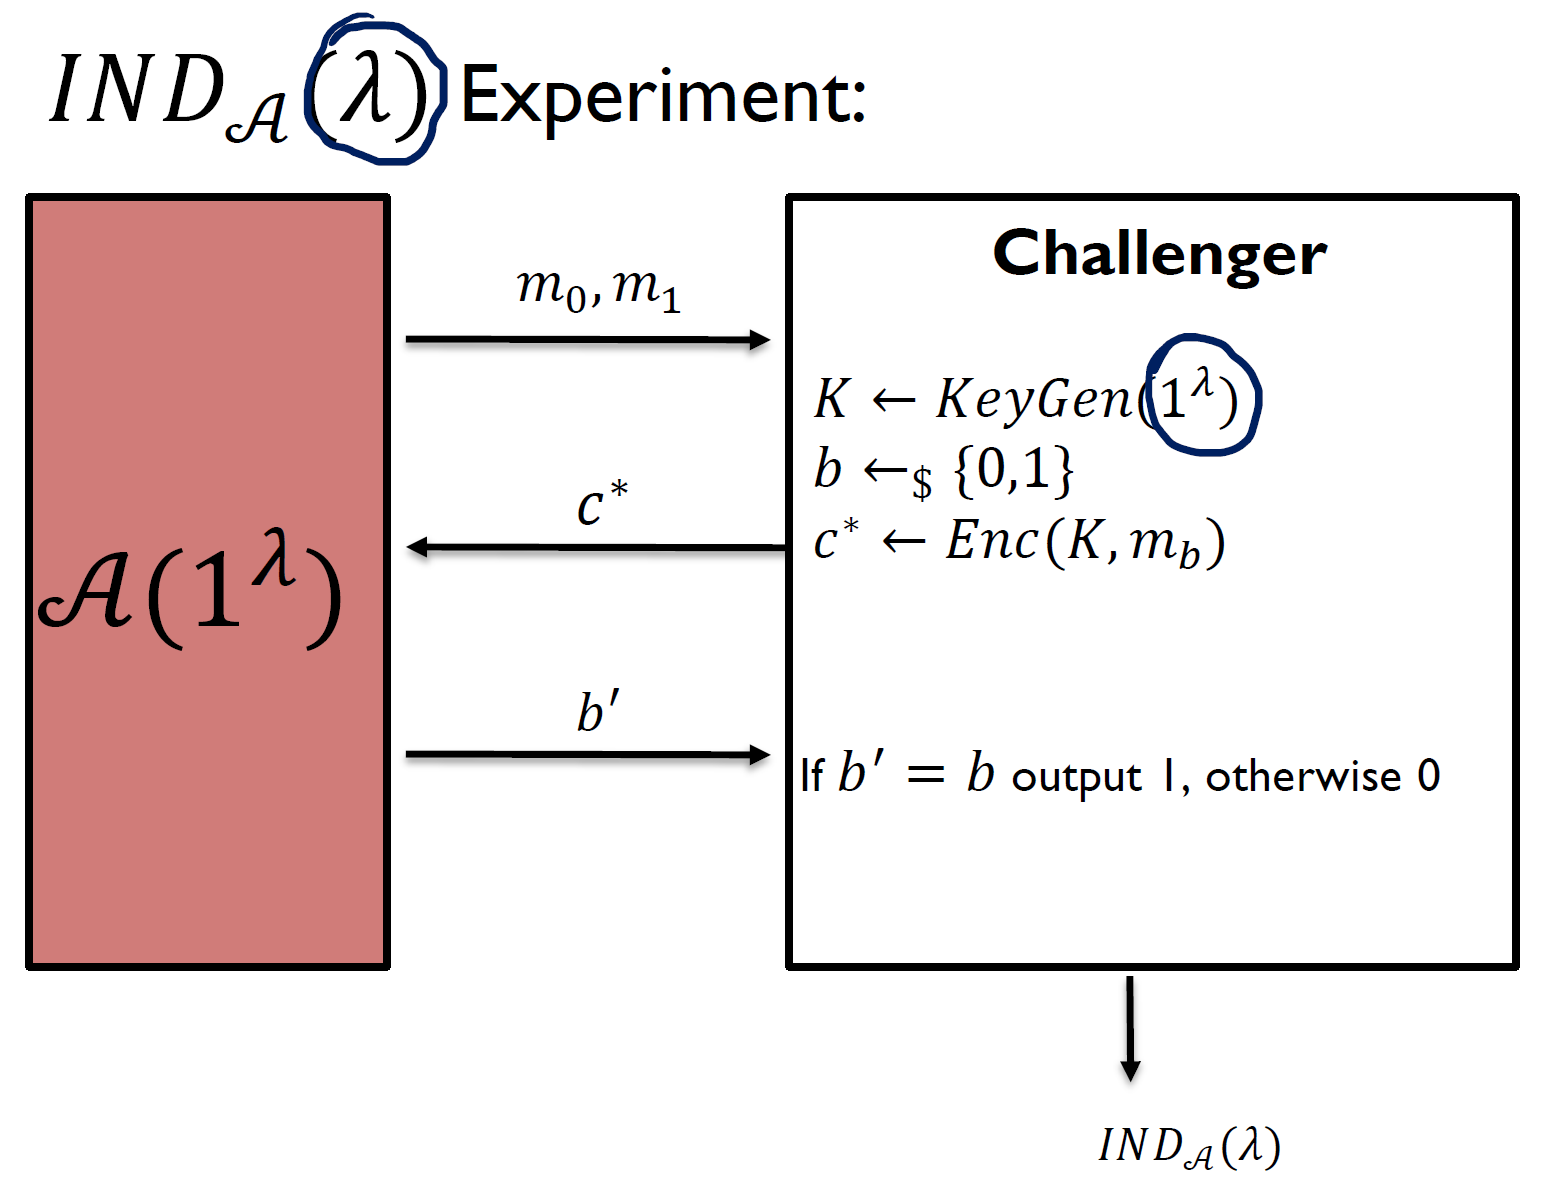
\includegraphics[width=140mm]{Graphics/Basics of Private Key Encryption/AsymptoticIndistinguishabilitySecurity.png}\newline
		\end{center}
	
	\section{Discussion}
		\begin{itemize}
			\item Asymptotic security allows us to base security of schemes on \textbf{standard assumptions} via reductions
			\item Shortcomings: Asymptotic security does not tell us how to instantiate schemes concretely
			\item But: Asymptotic security typically is a guarantee that a scheme has no design flaws.
			\item Attempt at reconciliation: \textit{Tight Security}, i.e. security reductions which provide concrete quantitative guarantees
		\end{itemize}
	
	\section{Summary}
		\begin{itemize}
			\item Perfect security is both an overkill and insufficient
			\item Computational Security: Only consider efficient adversaries, and require their advantage to be small
			\item Asymptotic security: efficient adversaries = \textbf{PPT algorithms}, small advantage = \textbf{negligible advantage}
		\end{itemize}





































